\documentclass[10pt]{llncs}
\pagestyle{plain}

\usepackage[cmex10]{amsmath}
\usepackage{amssymb}
\usepackage{array}
\usepackage{bm}
\usepackage{graphicx}
\usepackage{epstopdf}
\usepackage[hang]{subfigure}
\usepackage{import}
\usepackage{booktabs}
\usepackage{tabularx}
\usepackage{pdfpages}
\usepackage{epstopdf}
\graphicspath{{figures/}}
\usepackage{wrapfig}
\usepackage[export]{adjustbox}
\usepackage[font=scriptsize]{caption}



\usepackage[colorlinks=true,linkcolor=blue,citecolor=blue,urlcolor=black]{hyperref}
\usepackage{algorithm, algpseudocode}


% Commenting functionality
\usepackage{todonotes}
%\reversemarginpar

\newcommand{\brs}[1]{\left[{#1}\right]} %square bracets
\newcommand{\brr}[1]{{\left({#1}\right)}} %round bracets
\newcommand{\brf}[1]{\left\lbrace{#1}\right\rbrace} %figure bracets
\newcommand{\brabs}[1]{\left\vert{#1}\right\vert} %absolute bracets
\newcommand{\norm}[2]{\left\|{#1}\right\|_{#2}} %norm_*

\newcommand{\I}[1]{I\!\left[{#1}\right]} %Robustness criterion I[*]
\newcommand{\Iq}[1]{I_q\!\left[{#1}\right]} %Robustness criterion I_q[*]
\newcommand{\Ic}[1]{I_c\!\left[{#1}\right]} %Robustness criterion I_c[*]

\newcommand{\vx}{\mathbf{x}} % vector x
\newcommand{\vX}{\mathbf{X}} % vector X
\newcommand{\vf}{\mathbf{f}} % vector f
\newcommand{\vz}{\mathbf{z}} % vector z
\newcommand{\vZ}{\mathbf{Z}} % vector Z
\newcommand{\vw}{\mathbf{w}} % vector w
\newcommand{\vd}{\mathbf{d}} % vector d
\newcommand{\vp}{\mathbf{p}} % vector p
\newcommand{\vP}{\mathbf{P}} % vector P
\newcommand{\vu}{\mathbf{u}} % vector u
\newcommand{\vU}{\mathbf{U}} % vector U
\newcommand{\DSet}{\mathcal{D}} % Set D
\newcommand{\NSet}{\mathcal{N}} % Set N
\newcommand{\XSet}{\mathcal{X}} % set X
\newcommand{\ZSet}{\mathcal{Z}} % set Z
\newcommand{\SSet}{\mathcal{S}} % set S
\newcommand{\ISet}{\mathcal{I}} % set I
\newcommand{\Pref}{\mathcal{P}} % Preferences set P

\DeclareMathOperator*{\argmin}{\arg\!\min}
\DeclareMathOperator*{\argmax}{\arg\!\max}


\begin{document}
\title{sParEGO -- A Hybrid Optimization Algorithm for Expensive Uncertain Many-Objective Optimization Problems}
\author{Robin C. Purshouse\inst{1} \and Shaul Salomon\inst{2} \and Daniel C. Oara\inst{1} \and Peter J. Fleming\inst{1}}
\institute{Department of Automatic Control and Systems Engineering\\ University of Sheffield\\ Mappin Street, Sheffield S1 3JD, UK\\ \email{\{r.purshouse,dcoara1,p.fleming\}@sheffield.ac.uk}
\and Department of Mechanical Engineering\\ ORT Braude College of Engineering, Karmiel, Israel\\ \email{shaulsal@braude.ac.il}}

\maketitle

\begin{abstract}
Designing complex engineered products requires expensive computational simulations. In this context design optimization using a limited budget (usually a budget of 250 to 500) to evaluate the candidate designs with high-fidelity simulations can be challenging even with high available resources. Solving the stochastic optimization problem, when uncertainty is taken into account, is more difficult even using the currents state of the art algorithms which iteratively computes a surrogate model of the problem and use this model to guide the search for the best location for a new candidate design to be evaluated. This work introduces a new algorithm sParEGO - stochastic ParEGO, which is a extension of Knowles ParEGO algorithm \cite{Knowles2006ParEGO} to consider evaluation functions as samples of random variates. To test the results of the algorithm two situational test problems have been developed using a toolkit for generating stochastic multi-objective test problems presented by Shaul et al. at Gecco 2006.    

    
\keywords{Expensive optimization, surrogate-based optimization, robust optimization}
\end{abstract}

\section{\label{sec:intro}Introduction}
The algorithm for robust design optimization, is aimed at design activities involving
multiple objectives and featuring uncertainties of various sources. This framework intends to support the goal of a ``right-first-time-design", where appropriate design choices are made based on computer simulations alone. In this context, a high quality solution does not necessarily have to demonstrate the very best possible performance under a single set of assumptions, but rather to perform well under a large variety of uncertain factors.

\todo{Just something to work with. Obviously this needs to be rewritten}A general single-objective robust optimisation problem can be formulated as:
\begin{align}
\label{eq:rev:robust}
\min_{\vx\in\Omega} S=\vf\brr{\vx,\vU}.
\end{align}
Here, $\vU$ is a vector of random variables that includes all the uncertainties associated with the optimisation problem.
These uncertainties may be an outcome of manufacturing tolerances, a noisy environment, evaluation inaccuracies, and so on.
A single scenario of the variate $\vU$ is denoted as $\vu$.
Since uncertainties are involved, the scalar objective $S$ is also a random variate, where every scenario of the uncertainties, $\vu$, is associated with an objective value $s$.

In a robust optimisation scheme, the random objective value is replaced with a robustness criterion, denoted by the indicator $\I{S}$.
Several criteria are commonly used in the literature, which can be broadly categorised into three main approaches:
\begin{enumerate}
%
\item \textbf{Worst-Case Scenario.} The worst objective vector, considering a bounded domain in the neighbourhood of the nominal values of the uncertain variables.
%
\item \textbf{Aggregated Value.} An integral measure of robustness that amalgamates the possible values of the uncertain variables (e.g. mean value or variance).
%
\item \textbf{Threshold Probability.} The probability for the objective function to be better than a defined threshold.
\end{enumerate}

In this framework the third approach, suggested by Beyer and Sendhof~\cite{Beyer2007}, is used.
A threshold $q$ is considered as a satisfying performance for the objective value $s$.
When $s$ is uncertain, denoted by the random variable $S$, the probability for $S$ to satisfy the threshold level can be seen as a confidence level $c$.
For a minimization problem this can be written as:
\begin{align}
\label{eq:confidence}
	c\brr{S,q}=\text{Pr}\brr{S<q}.
\end{align}
Equation~\eqref{eq:confidence} can be used for two different robustness indicators:
\begin{enumerate}
	\item Minimization of the threshold $q$ for a pre-defined confidence level $c$, denoted as $\Ic{\bullet}$.
		This is useful when there is no specific target for performance, but the confidence in the resulting performance can be specified.
		The preferred solution is the one that guarantees the best performance with the specified confidence.
	\item Maximization of the confidence level $c$ for a given threshold $q$, denoted as $\Iq{\bullet}$.
		This measure can be used when the target for performance is known, and the emphasis is on meeting this target, rather than performing as well as possible.
\end{enumerate}


The algorithm focuses on the following stochastic unconstrained multiobjective optimization problem (MOP):
\begin{align}
\label{eq:mop}
	\min_{\vx\in\Omega} \vZ=\vf\brr{\vx, \vU},
\end{align}
where $\vx$ is a vector of $n_x$ decision variables in a feasible domain $\Omega$, $\vZ$ is a multivariate random vector of $n_z$ performance criteria and $\vf$ is a set of functions mapping from decision-space to objective-space:
\begin{align}
	\vf: \mathbb{R}^{n_x} \rightarrow \mathbb{R}^{n_z}.
\end{align}
Due to uncertainties over the problem parameters or the mapping functions themselves, every evaluation of the same decision vector may result in a different realisation of the objective vector $\vz$.
If some of the objectives are in conflict with one another, the solution to~\eqref{eq:mop} is expected to be a set of decision vectors, offering different trade-offs between the objectives.

\subsection{\label{sec:intro}Background}

The ability of numerical simulations to predict the performance of a candidate
design is constantly increasing. While some simulations can produce high-fidelity outputs relatively quickly, a typical mesh-based simulation can run for several hours, and even days. Even if a design team has access to supercomputing resources, the extensive run-time still implies that perhaps only a few hundred candidate designs can be explored using high-fidelity modelling resources. Unfortunately, conventional multi-objective optimization algorithms,
such as NSGA-II \cite{deb2002fast}, implemented in commercial packages typically require tens
of thousands of function evaluations to converge on a high quality solution \cite{hansen2010comparing,zhou2011multiobjective}. Therefore, the search for a promising design using expensive evaluation functions on a limited computational budget poses a great challenge.

To exacerbate this problem, optimizing for a robust solution is itself a computationally
demanding task. In order to gain confidence over the robustness of a solution to uncertainties, the statistical properties of the expected solution's performance must be quantised. In a world where the complexity of the high-fidelity models essentially produces a black-box mapping of inputs to outputs,such statistical properties would typically be found through repeated evaluation of the same solution using those high-fidelity models. Such Monte Carlo
sampling of a single candidate design is computationally expensive.

The framework we have developed aims to address these challenges for a single optimization node, situated within a wider family of nodes simultaneously working on the design of a complex engineered product. From the single-node perspective, the key characteristics of the problem formulation can be summarised as follows: 
\begin{itemize}
	\item Expensive, black-box evaluation functions for a candidate design
	\item Many objectives to be addressed simultaneously (i.e. more than three)
	\item Multiple sources of uncertainty:
		\begin{itemize}
			\item Fidelity of evaluation functions
			\item Manufacturing tolerances
			\item Inherent variation of operating conditions
			\item Uncertainty over the state of shared or coupled design choices
		\end{itemize}
	\item Interaction with a designer or decision facilitator:
		\begin{itemize}
			\item Working with robustness metrics to provide an understanding of the risk and 						  opportunity trade-offs between candidate designs
			\item Working with user preferences to steer the search towards a desirable 				 	 		  compromise solution.
		\end{itemize}
\end{itemize}


\section{sParEGO}
The main idea is that the uncertain distribution in objective space of every candidate solution is not quantified through Monte-Carlo sampling\footnote{or other uncertainty quantification methods such as polynomial Chaos}, but every solution is evaluated once, and the distribution is approximated based on the performance of nearby solutions.

A pseudo-code of sParEGO is presented in Algorithm~\ref{alg:sParEGO}.
Its stages are explained in details at the remaining of this section.

\begin{algorithm}
\caption{\textsc{sParEGO} Pseudo-code}
\label{alg:sParEGO}
\begin{algorithmic}[1]
	\Statex \textbf{Parameters:} initial set size $n_\text{init}$, robustness criterion $I$, \Comment{Section~\ref{subsec:Parameters}}
	\Statex \hspace{20mm} evaluation functions $\vf$, neighbourhood distance $\delta$,
	\Statex \hspace{20mm} number of reference direction vectors $n_d$
	\State $\DSet \leftarrow$ \textsc{SimplexLattice}($n_d$) \Comment{Secton~\ref{subsec:Simplex Lattice}}
	\State $\XSet \leftarrow$ initialise a set with neighbourhoods of solutions \Comment{Section~\ref{subsec:initialisation}}
	\State $\ZSet \leftarrow \vf\brr{\XSet}$ \Comment{evaluate the initial set}
	\While{stopping criteria not satisfied}
		\State Shuffle the set $\DSet$
		\ForAll{$\vd\in\DSet$}
			\ForAll{$\vx^i\in\XSet$}
				\State update neighbourhood $\NSet^i$ \Comment{Section~\ref{subsec:Uncertainty quantification}}
			\EndFor
			\State update ideal and nadir vectors
			\State $\SSet \leftarrow$ calculate scalar fitness value of all solutions \Comment{Section~\ref{subsec:Scalarising}}
			\State $\ISet \leftarrow \emptyset$
			\ForAll{$\vx^i\in\XSet$}
				\State approximate the distribution of $S^i$ \Comment{Section~\ref{subsec:Uncertainty quantification}}
				\State calculate robustness indicator $\I{S^i}$ \Comment{Section~\ref{subsec:robustness indicators}}
				\State $\ISet \leftarrow \ISet \cup \I{S^i}$
			\EndFor
			\State $model \leftarrow$ fit a Kriging model to the indicator values $\ISet$ \Comment{Section~\ref{subsec:Kriging}}
			\State $\vx^\text{new} \leftarrow$ maximize the expected improvement based on $model$
			\State $\vx^\text{pert} \leftarrow$ add a neighbour to $\vx^\text{new}$ \Comment{Section~\ref{subsec:Kriging}} 
			\State $\XSet \leftarrow \XSet \cup \brf{\vx^\text{new}, \vx^\text{pert}}$
			\State $\ZSet \leftarrow \ZSet \cup \brf{\vf\brr{\vx^\text{new}}, \vf\brr{\vx^\text{pert}}}$ \Comment{evaluate the new solutions}
		\EndFor
	\EndWhile
%\Statex
\end{algorithmic}
\end{algorithm}

\subsection{Parameters}
\label{subsec:Parameters}
\begin{itemize}
\item $\delta$ -- Neighbourhood distance.
Maximum Euclidean distance between solutions, in normalised decision space, to be considered as neighbours.
Default value is $0.1 \sqrt{n_x}$.
\item $n_\text{init}$ -- Size of initial population.
\item $n_\text{indp}$ -- Portion solutions in the initial population that are independently generated.
Must be smaller or equal to $n_\text{init}/2$.
\item $\delta_\text{pert}$ -- maximum distance between newly generated solutions.
Default value is $\delta / 2$.
\item $n_d$ -- Number of sub-problems for decomposition (number of reference direction vectors).
\item Scalarisation function. The norm $p$ when using weighted $Lp$ scalarisation.
\item $c$ -- Desired level of confidence in the performance of the solutions.
\item $\alpha$ -- Level of confidence in parameters of the sampled distribution. Default is $c$.
\item $\beta$ -- Bandwidth of the Kriging model. Defines the intensity of spatial correlation between solutions in the model. Default is $0.1 \delta$.
\item $n_\text{max}$ -- Maximum number of solutions to construct the Kriging model.
\end{itemize}

\subsection{Decomposition}
\label{subsec:Simplex Lattice}

Similar to ParEGO, the multiobjective problem is decomposed into multiple single-objective problems, where at every iteration, a focus is given for a different ratio between the objectives.
However, there are two differences:
\begin{enumerate}
\item Instead of generating a set of uniformly distributed weight vectors, a set of uniformly distributed reference vectors in objective space (direction vectors) is used.
A weight vector is computed to every direction vector according to the Generalised Decomposition framework~\cite{giagkiozis2014generalized}.
\item The algorithm cycles through all direction vectors before revisiting each direction.
At the beginning of every cycle the order of the weights is shuffled.
\end{enumerate}

The decision variables and objectives are likely to be incommensurable, and therefore both decision-space and objective-space are normalised to non-dimensional units in the following manner:
\begin{align}
	\tilde{x}_i &= \frac{x_i - x^l_i}{x^u_i - x^l_i} , &i=1,\ldots,n_x,\\
	\tilde{z}_j &= \frac{z_j - z^*_j}{z^n_j - z^*_j} , &j=1,\ldots,n_z,
\end{align}
where $x^u_i$ and $x^l_i$ are the upper and lower boundaries of the $i^\text{th}$ decision variable, $z^n_j$ and $z^*_j$ are the $j^\text{th}$ components of the known nadir and ideal vectors\footnote{The ideal vector is composed of the best value of each objective.
The nadir vector is composed of the worst value of each objective amongst all Pareto optimal solutions.
Both vectors are estimated according to the current available information concerning the objective-space.}, and the tilde accent represents a normalised, dimensionless variable.
The normalised values are used for all operations within the algorithm.
Before a candidate design is evaluated, it is re-scaled to the natural dimensions.

\subsubsection{Set of Reference Direction Vectors}
The multiobjective optimization problem is decomposed to $n$ sub-problems as described in Section~\ref{subsec:Scalarising}. Each sub-problem $i$ correspond to a reference direction vector $\vd_i$ from a set $\DSet$. In the case where no preference information exists, the set is constructed using a Simplex Lattice design~\cite{Scheffe1958Experiments}:
\begin{align}
	\label{eq:SimplexLattice}
	\begin{split}
		\DSet = \Biggl\lbrace\vd=\brs{d_1,\ldots,d_{n_z}}\quad \vert \quad &\sum_{j=1}^{n_z} d_j = 1 \quad \wedge \\
		& \forall j, \quad d_j = \frac{l}{h}, l\in\brf{0,\ldots,h} \Biggr\rbrace.
	\end{split}
\end{align}
The number of direction vectors, $n_d$, is determined by the dimensionality of the objective space, and the constant $h$: $\vert\DSet\vert = n_d = \binom{h+n_z-1}{n_z-1}$. The direction vectors are evenly distributed along the hyperplane $\sum d_j = 1$.

\subsection{Initialisation}
\label{subsec:initialisation}
To provide good initial coverage of potential designs, a space filling design (Latin hypercube) is used for the initial set.
However, the algorithm requires all solutions to reside within a distance of $\delta$ from other solutions (at least one).
To accomplish this, only $n_\text{indp} \leq n_\text{init}/2$ solutions are generated by Latin hypercube.
The rest of the solutions are generated as follows:
\begin{enumerate}
\item For every existing solution, another solution is randomly generated within a hypersphere with a radius of $\delta_\text{pert}$.
\item The rest of the solutions are generated by randomly selecting an existing solution and creating a nearby solution within a distance of $\delta_\text{pert}$.
\end{enumerate}
The first stage enforces that every solution has at least one neighbour.
The second stage seeds the initial population with neighbourhoods of different sizes.

\subsection{Scalarisation}
\label{subsec:Scalarising}
The scalarising function used in this framework is the popular \emph{weighted $L_p$}~\cite{koski1987norm,Marler2004Survey}:
\begin{align}
\label{eq:weighted Lp}
	s = \brr{\sum_{i=1}^{n_z} \brr{w_i\cdot \brr{z_i-z_i^*}}^p}^{1/p},
\end{align}
where $\mathbf{z^*}$ is a reference vector in objective space, typically the \emph{ideal} vector, which is composed of the minima of each individual objective.
For a given weighting vector $\vw$, a comparison between two vectors $\vz^{A}$ and $\vz^{B}$ depends on the choice of norm $p$. \todo{can refer to Naveed's EMO17 paper for the choice of norm}

For a given direction vector $\vd$ there is a corresponding weighting vector that minimizes the scalarising function \cite{giagkiozis2014generalized}. The optimal weighting vector $\mathbf{w}$ for the scalarising function in~\eqref{eq:weighted Lp} is defined as:
\begin{align}
\begin{split}
	&\mathbf{w}=\brs{w_1,\ldots,w_{n_z}},\\
	&w_i=a\cdot\brr{d_i+\epsilon}^{-1} \quad , \quad i=1,\ldots,n_z,\\
	&\sum_{i=1}^{n_z} w_i=1,
\end{split}
\end{align}
where $\epsilon$ is a small number to prevent division by zero, and $a$ is a normalisation factor.



\subsection{Uncertainty quantification}
\label{subsec:Uncertainty quantification}
The most important difference between sParEGO and ParEGO is that the former assumes that the outcome of an evaluation function is a realization of a random variate.
Therefore, the scalarised function value cannot be used directly to construct the surrogate model, and a utility indicator value is used instead.
For every direction vector $\vd$, the surrogate model is constructed to search for a design that will optimize a given robustness indicator (described later in Section~\ref{subsec:robustness indicators}).
The guiding principle is to avoid Monte Carlo methods that repeatedly sample every candidate design to assess its statistical properties in objective-space.
Instead, these properties (specifically, measures of central tendency and dispersion) are approximated from the available information of other candidate design evaluations.

\subsubsection{Approximation of the central tendency}
The stochasticity of the problem might originate from a variaety of sources, including variations in decision-space.
For this type of uncertainty, two designs with similar nominal values can be identical when realised.
Therefore, the performance of a candidate design should be calculated from the performance of neighbouring designs as well.
A distance\footnote{Distance is measured in decision-space by the Euclidean norm.} in normalised decision space $\delta$ is defined, such that two solutions $\vx^i$ and $\vx^j$ are considered as neighbours if:
\begin{align}
	\norm{\vx^i-\vx^j}{2}\leq\delta.
\end{align}
For a solution $\vx^i$, the statistical properties of the scalar fitness are approximated from the neighbouring solutions as follows:
First, the neighbourhood $\NSet^i$ of the solution is defined\footnote{Note that according to~\eqref{eq:neighbourhood}, $\vx^i$ is included in the neighbourhood $\NSet^i$.}:
\begin{align}
	\label{eq:neighbourhood}
	\NSet^i=\brf{\vx^j\in \XSet \,\vert \,\norm{\vx^i-\vx^j}{2}\leq\delta}.
\end{align}
Next, the approximated mean function value, $\mu_s$, is derived from the neighbourhood.
Members that are closer to $\vx^i$ are given a larger weight, denoted as $v$ in Equation~\eqref{eq:neighbourhood weights}, in approximating its properties.
Since the weight of most solutions in the neighbourhood is smaller than 1, the overall "neighbourhood size" $N^i$ is smaller than $\brabs{\NSet^i}$:
\begin{align}
	\label{eq:neighbourhood weights}
	v^j &= \frac{\delta-\norm{\vx^i-\vx^j}{2}}{\delta}, \quad  \forall \vx^j\in\NSet^i,\\
	\label{eq:neighbourhood size}
	N^i &= \sum_{\vx^j\in\NSet^i} v^j,\\
	\label{eq:neighbourhood mean}
	\mu^i_s &= \left. \sum_{\vx^j\in\NSet^i} v^j s^j \middle/ N^i \right. .
\end{align}

In Figure~\ref{subfig:indicator_estimation_1} the scalar fitness values of four candidate solutions (with a single decision variable) are depicted as grey dots.
The values of the expected mean $\mu_s\brr{x}$ are depicted as black dots.

\subsubsection{Approximation of the dispersion}
Once the expected mean is known, the expected value for the variance is calculated:
\begin{align}
	\label{eq:neighbourhood variance}	\sigma^{2,i}_s = \left. \sum_{\vx^j\in\NSet^i} v^j \brr{s^j - \mu^i_s}^2 \middle/ N^i \right. .
\end{align}
Since the variance in~\eqref{eq:neighbourhood variance} is calculated from a sample (possibly small), the standard error of the sample needs to be taken into account. \todo{consider leaving this part out}
This can be calculated from a chi-squared distribution with $N^i-1$ degrees of freedom.
For a confidence level $\alpha$ for the variance, the upper bound of the confidence interval is:
\begin{align}
	\label{eq:variance upper bound} \sigma^{\prime 2,i}_s = \frac{\sigma^{2,i}_s\brr{N^i-1}} {X^2_{1-\alpha/2}},
\end{align}
where $X^2_{1-\alpha/2}$ is the $1-\alpha/2$ percentile of a chi-squared distribution with $N-1$ degrees of freedom.
The intervals of $\mu_s\pm\sigma_s$ and $\mu_s\pm\sigma'_s$ are depicted in Figure~\ref{subfig:indicator_estimation_b} in red and blue, respectively.

\begin{figure}% 3D graphical demonstration
\centering
\subfigure[Estimation of the mean value and the variance from the neighbourhood]{
	\label{subfig:indicator_estimation_1}
	\def\svgwidth{0.45\textwidth}
	\import{figures/}{indicator_estimation_1.pdf_tex}
}
\hspace{2mm}
\subfigure[Assuming a normal distribution for $S$ according to $\mu_s$ and $\sigma_s$. The shaded area represents the a confidence of $80\%$.]{
	\label{subfig:indicator_estimation_2}
	\def\svgwidth{0.45\textwidth}
	\import{figures/}{indicator_estimation_2.pdf_tex}
}
\caption{\subref{subfig:indicator_estimation_a}-\subref{subfig:indicator_estimation_c} Approximation of the statistical properties. \subref{subfig:indicator_estimation_d} Calculation of robustness indicator $\Iq{\bullet}$.}
\label{fig:indicator_estimation}
%% label for entire figure
\end{figure}

\subsection{Estimating the robustness indicator value}
\label{subsec:robustness indicators}

Once the mean and variance of the scalar fitness function have been estimated for every solution in the set, the random variable $S\brr{\vx}$ is assumed to follow a normal distribution.
Given a desired confidence level $c$, the robustness indicator $\Ic{S}$ can be calculated.
An example for $\Ic{S}$ is given in Figure~\ref{subfig:indicator_estimation_2}.
The indicator value $\Ic{S}$ is considered as the solution's fitness at the current iteration.

\subsection{Fitting a Surrogate Model to the Fitness}
\label{subsec:Kriging}
Now that every solution is associated with a scalar fitness value, the algorithm proceeds in a similar fashion to EGO and ParEGO \cite{Jones1998Efficient,knowles2005multiobjective}.
A surrogate model is fitted to the fitness values, and the expected improvement function is constructed from the model and its prediction error.

For some \todo{replace ``some reasons'' with the actual reasons (if you know them)} reasons, instead of the DACE model used in EGO, here we constructed a Kriging model with a power variogram.
The model's bandwidth, $\beta$, affects the spatial correlation between samples.
It is advisable to set the bandwidth according the neighbourhood distance, $\delta$.
A relation of $\beta=0.1\delta$ has given good results on a set of preliminary tests.

Above a certain size (approximately 100 solutions), the Kriging model becomes prohibitively expensive to construct.
When the number of evaluated solutions exceed this size, a subset of size $n_\text{max}$ is is chosen according to Algorithm~\ref{alg:filtration}.

\begin{algorithm}
\caption{Choosing a Subset to Construct the Surrogate Model}
\label{alg:filtration}
\begin{algorithmic}[1]
	\Require population set $\XSet$, subset size $n_\text{max}$, current direction vector $\vd$
	\Ensure a subset $\XSet'$ of size $n_\text{max}$
	\State $\XSet' \leftarrow n_\text{max}/2$ solutions from $\XSet$ with the best indicator value
	\State $\XSet'' \leftarrow \XSet \setminus \XSet'$
	\ForAll{$\vx \in \XSet''$}
		\State $\hat{\vz}\brr{\vx} \leftarrow$ normalise $\vz\brr{\vx}$ and project it on the $k-1$ simplex
		\State $\Delta\brr{\vx, \vd} \leftarrow \norm{\hat{\vz}\brr{\vx} - \vd}{2}$
	\EndFor
	\State $\XSet' \leftarrow \XSet' \cup n_\text{max}/2$ solutions from $\XSet''$ with the smallest $\Delta$ distance
\end{algorithmic}
\end{algorithm}

\subsection{Optimization of the Expected Improvement}
A single objective global optimization algorithm is used to maximize the expected improvement.
Here we used an evolutionary algorithm ACROMUSE \cite{Ginley2011}.
Once a solution $\vx^\text{new}$ that maximizes the expected improvement is identified, it is added to the population together with a neighbouring solution $\vx^\text{pert}$, generated in a similar fashion to the initial solutions described in Section~\ref{subsec:initialisation}.

\section{Other aspects of the framework}
\label{sec:Other aspects}
\subsection{Attitude to risk}
\label{subsec:risk}
\todo{maybe we want to include this in the conclusions?}
In robust design optimization, there is an inherent trade-off between the solution's expected performance and the confidence in achieving it under extreme scenarios of the uncertainties involved. sParEGO provides four parameters to express the decision maker attitude to risk:
\begin{itemize}
	\item When the robustness metric $\Iq{\bullet}$ is used, the confidence level $c$ can be specified.
	\item When estimating the variance upper bound $\sigma^{\prime 2}_s$  in Equation~\eqref{eq:variance upper bound}, the confidence level $\alpha$ can be specified.
	\item The value used for approximating the variance of isolated solutions $\sigma^{\prime\prime 2}_s$ in Figure~\ref{subfig:indicator_estimation_c}, represents a risk averse attitude. A less conservative approach would be not to consider a smaller value than the upper bound of the model prediction interval.
	\item The value $\delta$--the maximum distance between solutions to be considered as neighbours--affects the variance of solutions and the convergence rate.
		For smooth and continuous functions, a tight neighbourhood is likely to result in smaller variance, but also uses less information from other solutions, which reduces convergence rate.
\end{itemize}

\begin{figure}
\centering
\def\svgwidth{0.45\textwidth}
\import{figures/}{convergence_hv.pdf_tex}
\caption{WE CAN USE THIS FIGURE TO EXPLAIN THE COMPARISON BETWEEN ParEGO AND sParEGO. OR DID WE USE THE PERCENTILES OF THE MARGINAL DISTRIBUTIONS?}
\label{fig:convergence}
\end{figure}


\section{Results}
\label{sec:results}

\begin{wrapfigure}{r}{0.5\textwidth}
\vspace{-80pt}
\begin{center}
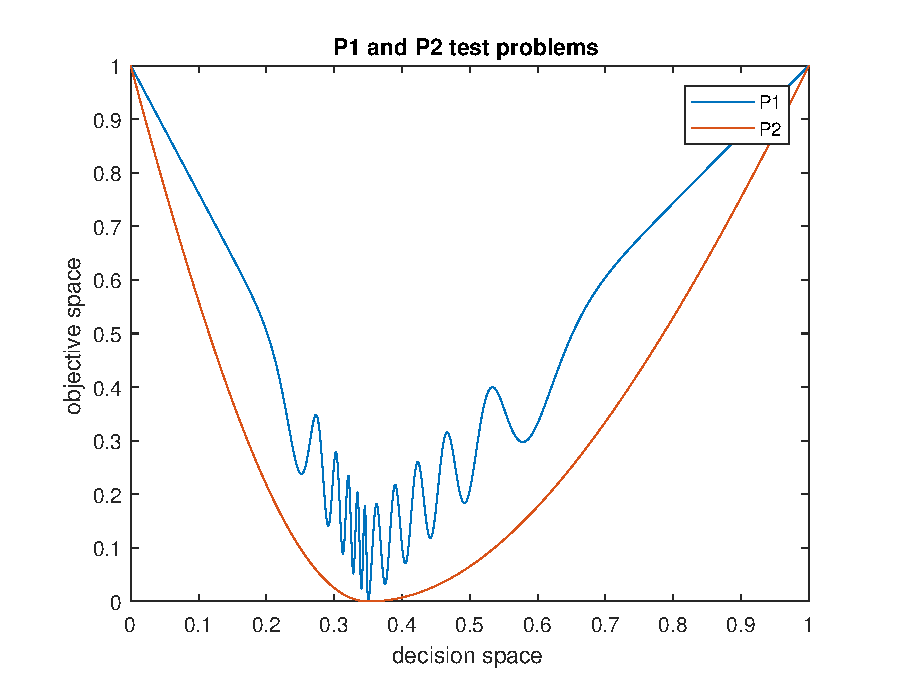
\includegraphics[scale=0.45]{testproblems}
\end{center}
\vspace{-20pt}
\caption{Test problems P1 and P2}
\vspace{-20pt}
\label{fig:TestProblems}
\end{wrapfigure}

To test the performance of sParEGO we propose two situational testing problems based on a toolkit for generating stochastic multiobjective test problems \cite{Salomon2016Toolkit}. The first test problem named P1 is a fist degree polynomial deterministic problem, multi-modal around the optima and with a smooth surface. The second test problem named P2 is a second degree polynomial stochastic problem and has no modality. The two test problems can be seen in Figure \ref{fig:TestProblems}.  


For both test problems sParEGO results have been compared with the ParEGO ones (being the state of the art algorithm for solving multi-objective optimization problems) using the same budget of 500 evaluation for a bi-objective problems with 5 decision variables, population size was 52 and the number of reference direction used was 11. Both ParEGO and sParEGO algorithms have been tested 21 times on each problem and the solution of the median run are presented in Figure \ref{fig:MedainRun} below.  
    
\begin{figure}[h]
\centering
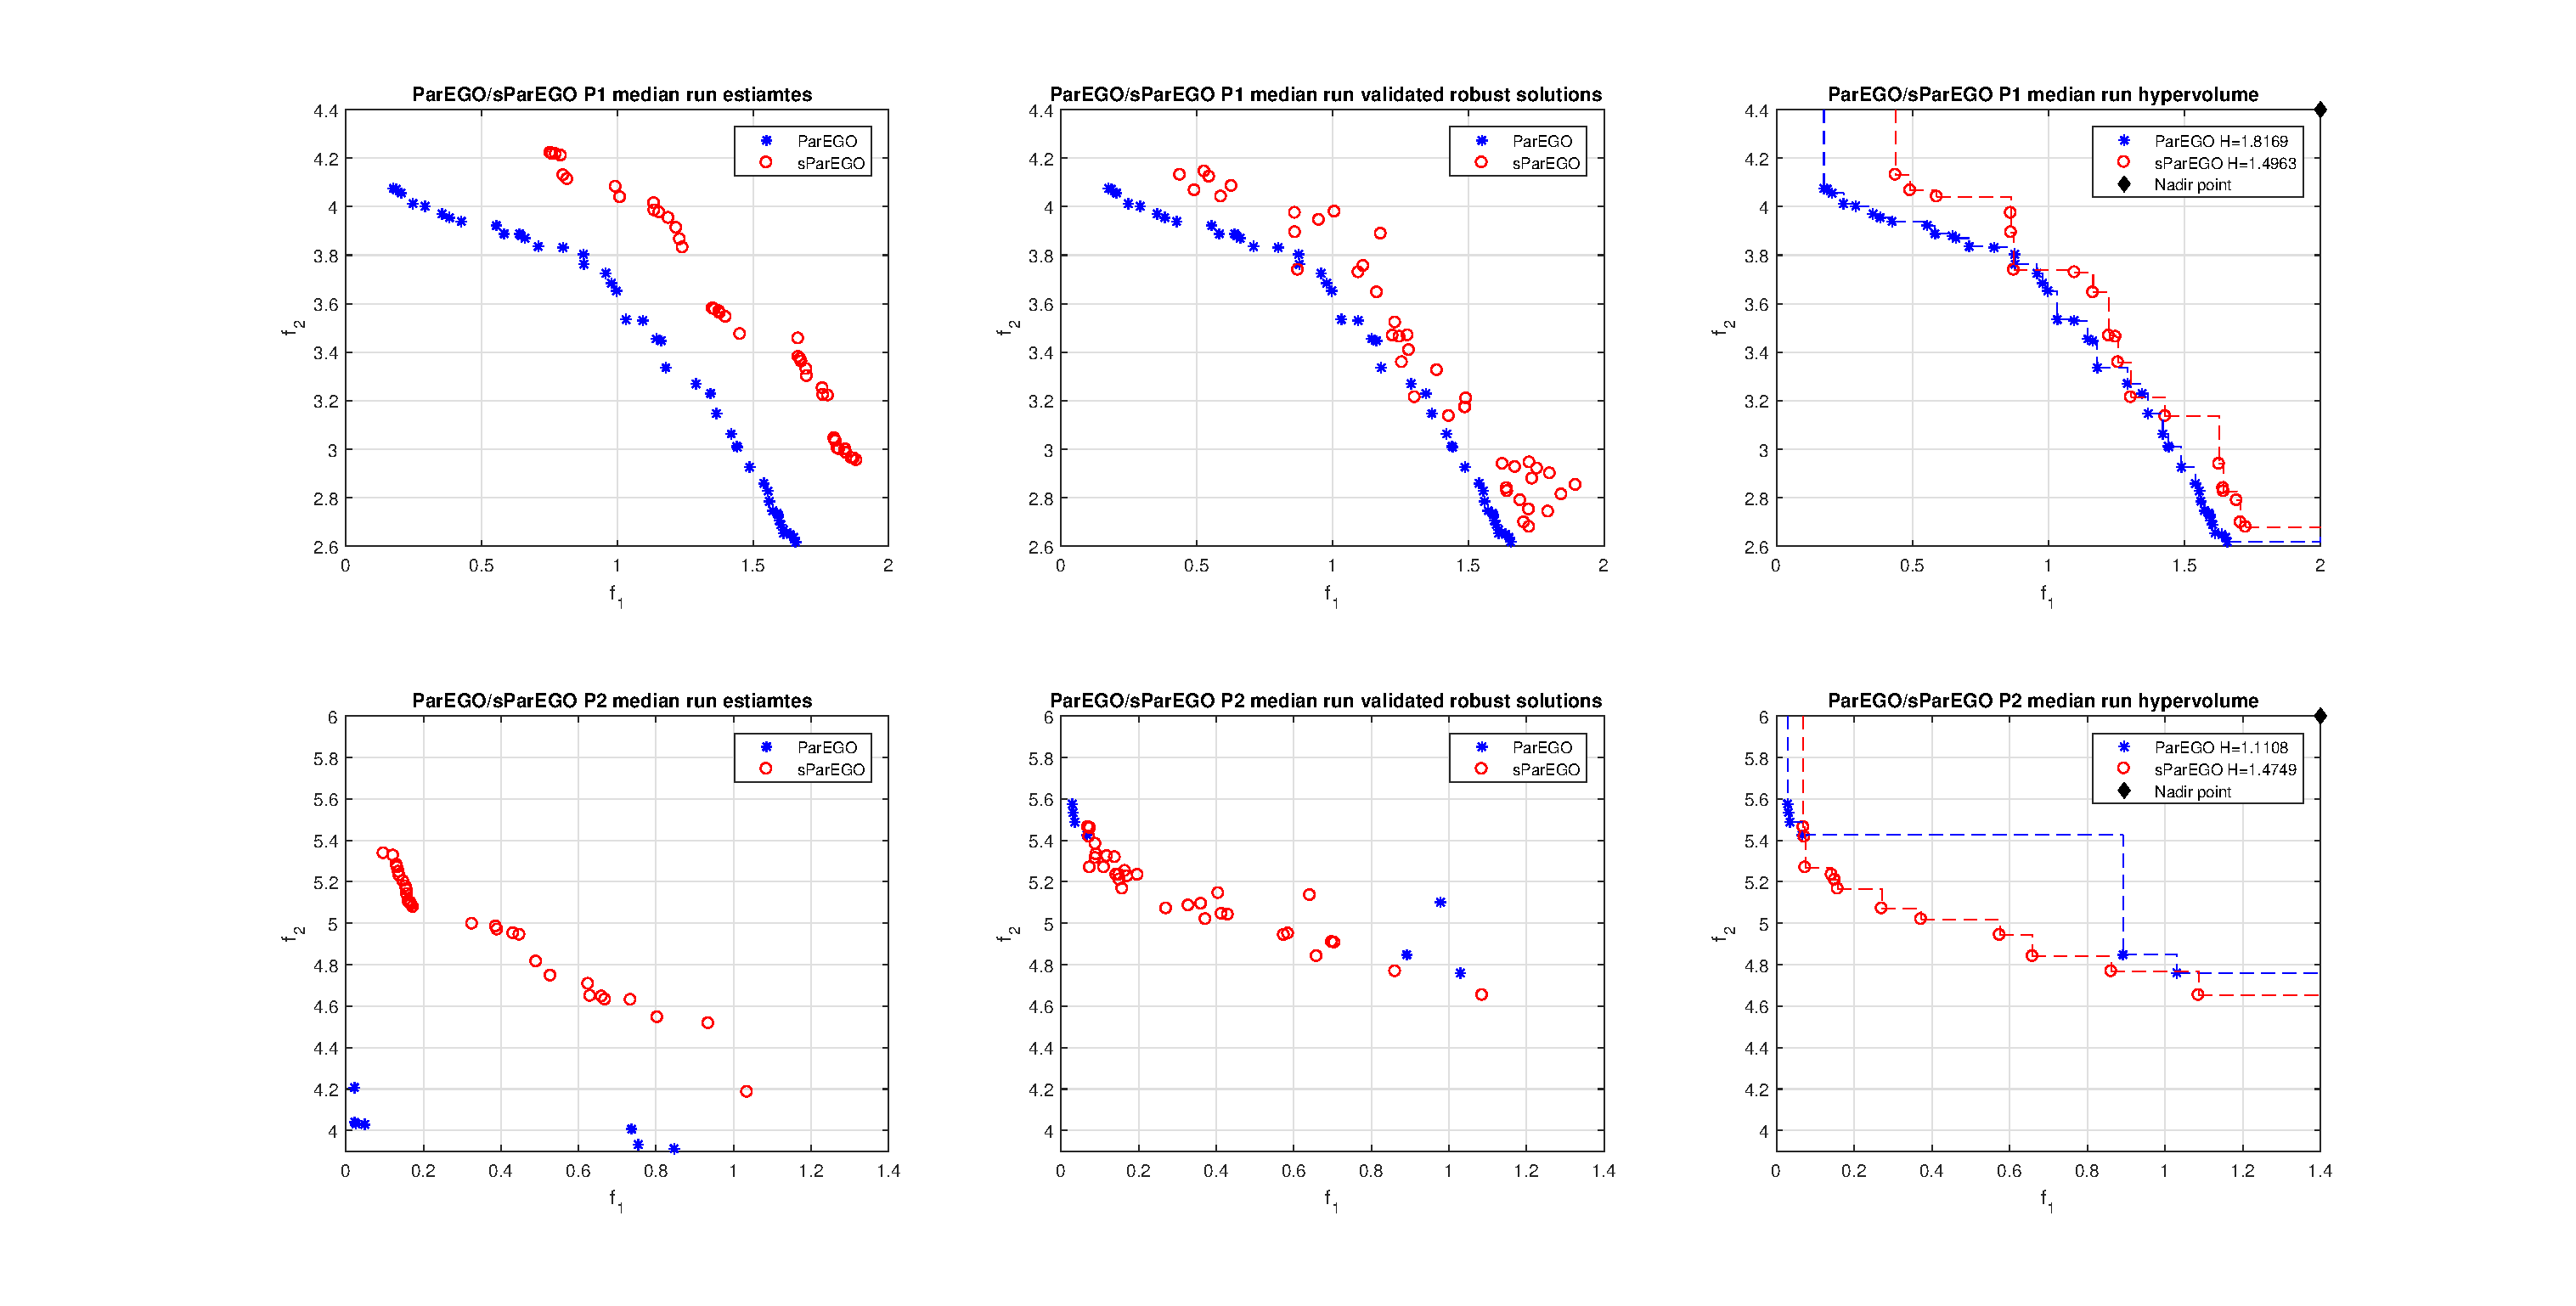
\includegraphics[width=1.5\textwidth, center]{P1P2}
\caption{Median run of test problems P1 and P2. Starting with the top left corner the median run estimates of the ParEGO and sParEGO algorithms for the first problem can be observed, followed by the graph of the 90 percentile Monte Carlo validation and in the top right corner is the Hypervolume measure of the validated robust solutions. The bottom of the figure presents the results of the second problems starting in the left with median run estimates of the ParEGO and sParEGO algorithms, followed by the 90 percentile Monte Carlo validation and in the bottom left corner is the Hypervolume measure of the validated robust solutions.}
\label{fig:MedainRun}
\end{figure}

In Figure \ref{fig:MedainRun} can be observed in the top graphs the result of the P1 test problem. The problem is deterministic and ParEGO manage to find the pareto front with a better accuracy than sParEGO, as sParEGO is designed to be more restrictive and find robust solutions. This can be confirmed by the Monte Carlo validation, the sParEGO result are better that the estimates and come closer to the pareto front. The last figure in the first top right corner presents the Hypervolume measure of both algorithms for the median run.

On the Figure \ref{fig:MedainRun} bottom graphs are the results of the P2 test problem. Can be seen in the bottom left one that the ParEGO estimates can not find the pareto front because of the uncertainty in the problem formulation, as close you get to the pareto front more uncertainty will be present. sParEGO in the other hand manage to be closer to the pareto front as the second graphs confirms by validation using Monte Carlo and tating the 90 percentile of the distribution. In the last bottom right figure the hypervolume measure of both algortims is presented. From here can be concluded that sParEGO finds a better approximation of the robust pareto front, therefore using sParEGO in solving stochastic multiobjective optimization problems will give to the decision maker estimates that are closer to the true solutions and by validating the selected design the true performance can be recorded.
    
Figure \ref{fig:EI} illustrates the Expected Improvement results for the ParEGO in the left graphs for the P1$\&$P2  problems  and sParEGO in the right graphs. The lines represents the improvement on each reference direction over the number of evaluations. The number of reference direction was set to 11 and the budget for both algorithms was set to 500. 

\begin{figure}
\begin{center}
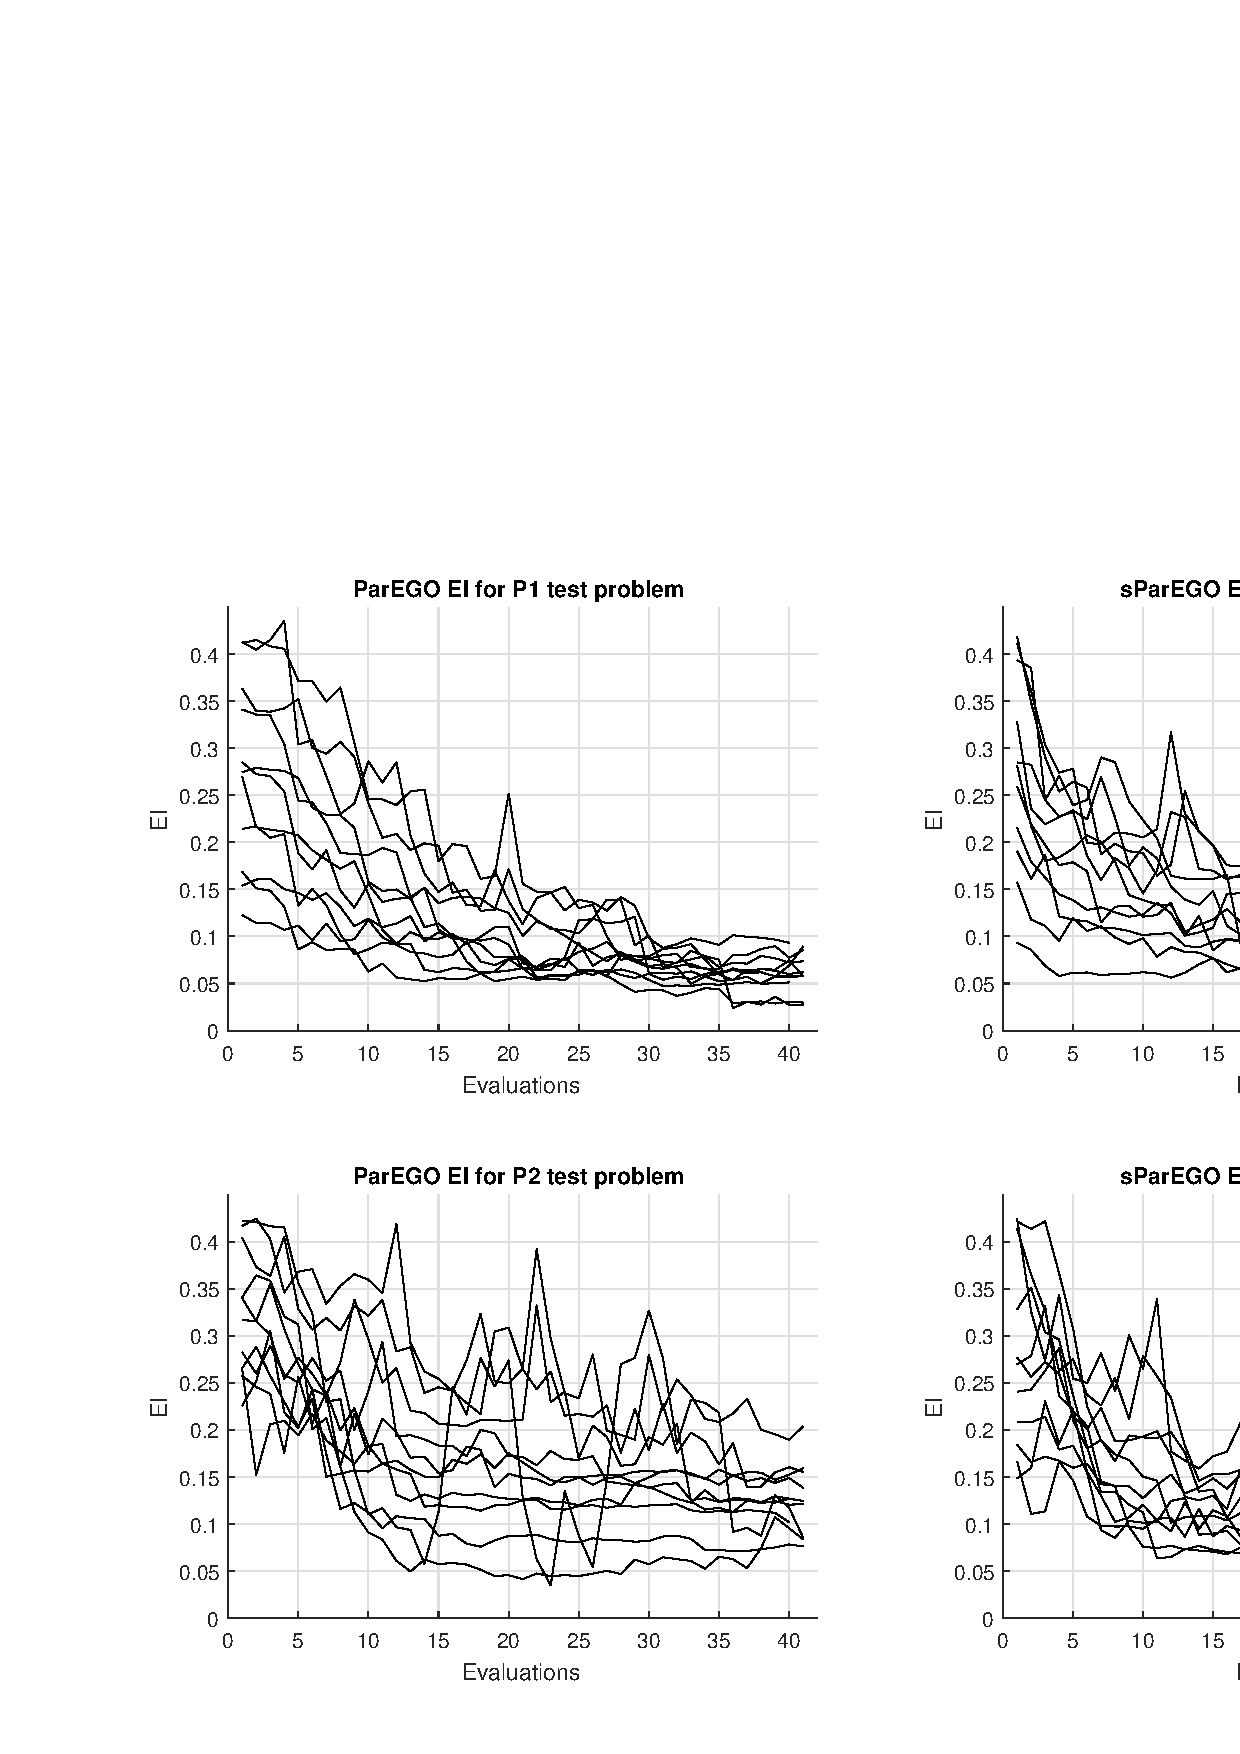
\includegraphics[scale=0.45, center]{EI}
\end{center}
\caption{Expected Improvement of the P1 and P2 problems. Starting with the top figures in the left the ParEGO EI for each reference direction can be seen how it is improving over the number of evaluations, and the right sParEGO EI value are presented for the first test problem. Followed below by the results of the second test problem in the left for ParEGO and the right for sParEGO.}
\label{fig:EI}
\end{figure}





\section{Conclusion}
\label{sec:conclusion}

\subsection{Framework limitations and risks}
This section summarises the assumptions made within the framework described in this document, and the risks associated with these assumptions.
\begin{itemize}
	\item \emph{The landscape is well behaved (i.e., smooth, continuous).} The uncertainty distributions are approximated according to available information for other candidate solutions. The underlying assumption for approximating in this way is that similar solutions have similar performance. If the functions are highly ragged and discontinuous, the surrogate models cannot accurately predict their behaviour.
	\item \emph{The dimensionality is small to medium.} The search is conducted on a surrogate model fitted to the existing evaluated solutions. The DACE model used in this framework typically produces good estimates for problems with up to 20 design variables.
	\item \emph{The problem formulation is appropriately elicited.} The outcomes from any use of the framework can only be as good as the information provided to it. Methodologies for robustly eliciting the problem formulation lie outside the scope of the project.
\end{itemize}


\bibliographystyle{splncs}
\bibliography{sparegoReferences}

\end{document}